\section{Measurement of muon (g-2) and EDM with reaccelerated thermal muon}

%\subsection{Principle of Measurements}\label{sec:Principle} 

%The current experimental result for $a_{\mu}$ was from the E821 experiment 
%at Brookhaven National Laboratory~\cite{Bennett:2006fi}, 
%which used the ``magic gamma" approach with 100\% polarized 3~GeV muons 
%injected by an inflector magnet with 2-5\% efficiency into a 14 meter diameter 
%storage ring built with 360~degree superconducting coils, 
%12 iron back-leg sectors and 36 iron pole sectors. 
%With iron shims, a 1 part per million (ppm) field uniformity was achieved after
%averaged over the muon orbit, with local non-uniformity of up to 100~ppm. 
%Electrostatic focusing was used in the ring, and decay positrons (and electrons) 
%were observed with calorimetry.  A new measurement of $a_{\mu}$ is underway 
%at Fermilab~\cite{Grange:2015fou}, using the BNL-E821 14~meter diameter storage ring,
%with a new muon accumulator ring and significant magnetic shimming improvements, 
%with expected improvements in statistical and systematic uncertainties.

%The experiment introduced here
%is intended to measure $a_{\mu}$ and $d_{\mu}$ with a very different technique,
%using 300~MeV/$c$ reaccelerated thermal muon beam with 50\% polarization,
%vertically injected into a MRI-type 66~cm diameter solenoid storage ring 
%with 1~ppm local uniformity for the storage magnetic field.
%The vertical injection, invented for this experiment, 
%will improve injection efficiency by more than an order of magnitude.
%Very weak magnetic focusing will be used in the ring. 
%Silicon strip detectors in the field will measure 
%the momentum vector of the decay positrons. 

%Table~\ref{T:Comparison} compares the proposed experiment with the previous
%experiment BNL-E821, and the current experiment Fermilab-E989.
%The initial goal of this experiment is to reach the statistical uncertainty for $a_{\mu}$ 
%of BNL-E821, with much smaller systematic uncertainties from sources different from the current method.
%The muon EDM goal is a statistical sensitivity of $1.4\times 10^{-21}~e\cdot\mbox{cm}$
%with a systematic uncertainties of $0.36\times 10^{-21}~e\cdot\mbox{cm}$,
%which is a factor 60 improvement over the present limit~\cite{Bennett:2008dy}.

The muon anomalous magnetic moment $a_{\mu}$ and electric dipole moment $d_{\mu}$ are defined as 
\begin{equation}
a_{\mu} = \frac{g-2}{2} ~~~ {\rm with} ~~~~ \vec{\mu} = g \left( \frac{e}{2m}
                  \right) \vec{s}, ~~~~
\vec{d} = \eta \left( \frac{e}{2mc}
                  \right) \vec{s},
\end{equation}
where $e, m$ and $\vec{s}$ are the electric charge, mass, and spin vector of muon, respectively.
Here, $g$ is the Land\'e's $g$ factor and $\eta$ is a corresponding factor for EDM.
Experiments measures spin precession of polarized muons under magnetic field.
Garwin \textit{et al.} found the overved rate of spin precession for stopped muon gave $g = 2.0 \pm 0.10$~\cite{Garwin:1957hc}, 
followed by more accurate measurement to ovserve the anomalous magnetic moment $a_{\mu}=(1.12 \pm 0.16)\times 10^{-3}$~\cite{Garwin:1960zz}.
Since then, experiments at CERN~\cite{Charpak:1961mz,Bailey:1969pr,Bailey:1975qi,Bailey:1978mn} 
store spin polarized muon beam in magnetic field to gain direct sensitivity to $a_{\mu}$.
Spin of the stored muon precesses, while muons make a cyclotron motion under the magnetic field.
With the non-zero and positive value for $g-2$, the spin direction makes a slow rotation 
with respect to the momentum direction.
The spin precession vector with respect to its momentum 
in static magnetic field $\vec{B}$ and electric field $\vec{E}$
is given as~\cite{Thomas1927,PhysRevLett.2.435,PhysRevLett.2.492,Khriplovich:1998zq,Fukuyama:2013ioa,Fukuyama:2018nbl}.

\begin{eqnarray} 
\vec{\omega} & = & \vec{\omega}_{a} + \vec{\omega}_{\eta} \\ 
             & = & 
  - \frac{e}{m}\left[a_{\mu} \vec{B} - 
   \left( a_{\mu}- \frac{1}{\gamma^2-1} \right)
   \frac{\vec{\beta} \times \vec{E}}{c}
  +\frac{\eta}{2} 
   \left(\vec{\beta} \times \vec{B}  + \frac{\vec{E}}{c}
   \right)
   \right].
\label{eq:omega_full}
\end{eqnarray}
Here $\vec{\omega}_{a}$ and $\vec{\omega}_{\eta}$ are precession vectors
due to $g-2$ and EDM. $\vec{\beta}$ and $\gamma$ are velocity and Lorentz factor of muon,
respectively.

In the measurements at CERN, BNL~\cite{Bennett:2006fi},
and Fermilab~\cite{Grange:2015fou}, the energy of the muon
was chosen to cancel the term of $\vec{\beta} \times \vec{E}$,
which allowed for electrostatic focusing in the storage ring 
without affecting the muon spin precession to first order. 
A focusing field index of $n =$0.12--0.14 was used in the BNL experiment
to keep the muons in the storage magnetic field.

A new experiment at J-PARC~\cite{TDRsummarypaper} plans to reduce the focusing requirement 
in the storage ring by using the reaccelerated thermal muon beam with a small transverse beam 
emittance $\sim1\pi$~mm$\cdot$mrad.
With such a beam, muons can be stored with a weak focusing magnetic field 
with a field index of $n \sim 10^{-4}$ without having electric field.
Under this condition, Eq.~(\ref{eq:omega_full}) reduces to
\begin{equation}
\vec{\omega}  =  
  - \frac{e}{m}\left[a_{\mu} \vec{B} 
  +\frac{\eta}{2} 
   \left(\vec{\beta} \times \vec{B} \right) 
   \right].
\label{eq:omega_tot}
\end{equation}
There is no contribution from the $\vec{\beta} \times \vec{E}$ term at any beam energy.
Since the precession vectors $\vec{\omega}_{a}$ and $\vec{\omega}_{\eta}$ 
are orthogonal each other, the $g-2$ and EDM precessions 
can be measured simultaneously with
an appropriate detector design.

The key requirement for this new approach to the measurement is a muon beam with low emittance.
This can be realized by a source of 
thermal energy positive muons followed by
reacceleration, without changing the transerse momentum spread. 
We note here that the stopping muons and their reacceleration steps will also
allow us to frequently reverse the muon spins by using static electro-magnetic fields.
This feature will be a powerful tool to study
rate-dependent systematics such as track reconstruction efficiency, and the effect on pile-up hits.

In the extraction of $a_{\mu}$ and $\eta$, 
the precession frequency $\vec{\omega}$ and the magnetic field $B$ must
be measured. The $\vec{\omega}$ is measured by detecting positrons from muon decay during the storage.
Since higher energy $e^+$ are emitted with the muon spin direction 
aligned with its motion~\cite{Konopinski:1959qr}, the number of high energy $e^+$ will show 
an oscillation in time as the muon spin precesses from forward to backward 
with respect to the muon momentum direction.
Detectors located radially inside the muon storage orbit will track the decay
$e^{+}$. The experiment records the number of higher energy $e^{+}$ 
versus time in storage, as the muon spin precesses in the magnetic field.

The average magnetic field seen by the muons in the storage ring 
is measured by the Larmor precession frequency of a free proton ($\omega_p$).
This is obtained from a convolution of the magnetic field map
and the muon beam distribution measured by the experiment.

Assuming the EDM term is negligibly small compared with the $g-2$ term in Eq.~(\ref{eq:omega_tot}), 
$a_\mu$ is obtained from 
$\omega_a = \frac{e}{m} a_\mu B$.
By using $\omega_p$, one can rewrite this equation to
\begin{eqnarray}
a_\mu = \frac{R}{\lambda - R},
\label{eq:amu}
\end{eqnarray}
where $R = \omega_a /\omega_p$ and $\lambda = \mu_\mu/\mu_p$ is the muon-to-proton
magnetic moment ratio externally provided.
The precision of the direct measurement of $\lambda$ by muonium spectroscopy in magnetic field
is 120~ppb~\cite{Liu:1999iz}. 
A new improved measurement of $\lambda$ is being prepared at J-PARC MLF in the same beamline~\cite{Shimomura:2015aza}.

\begin{figure}[t]
  \begin{center}
      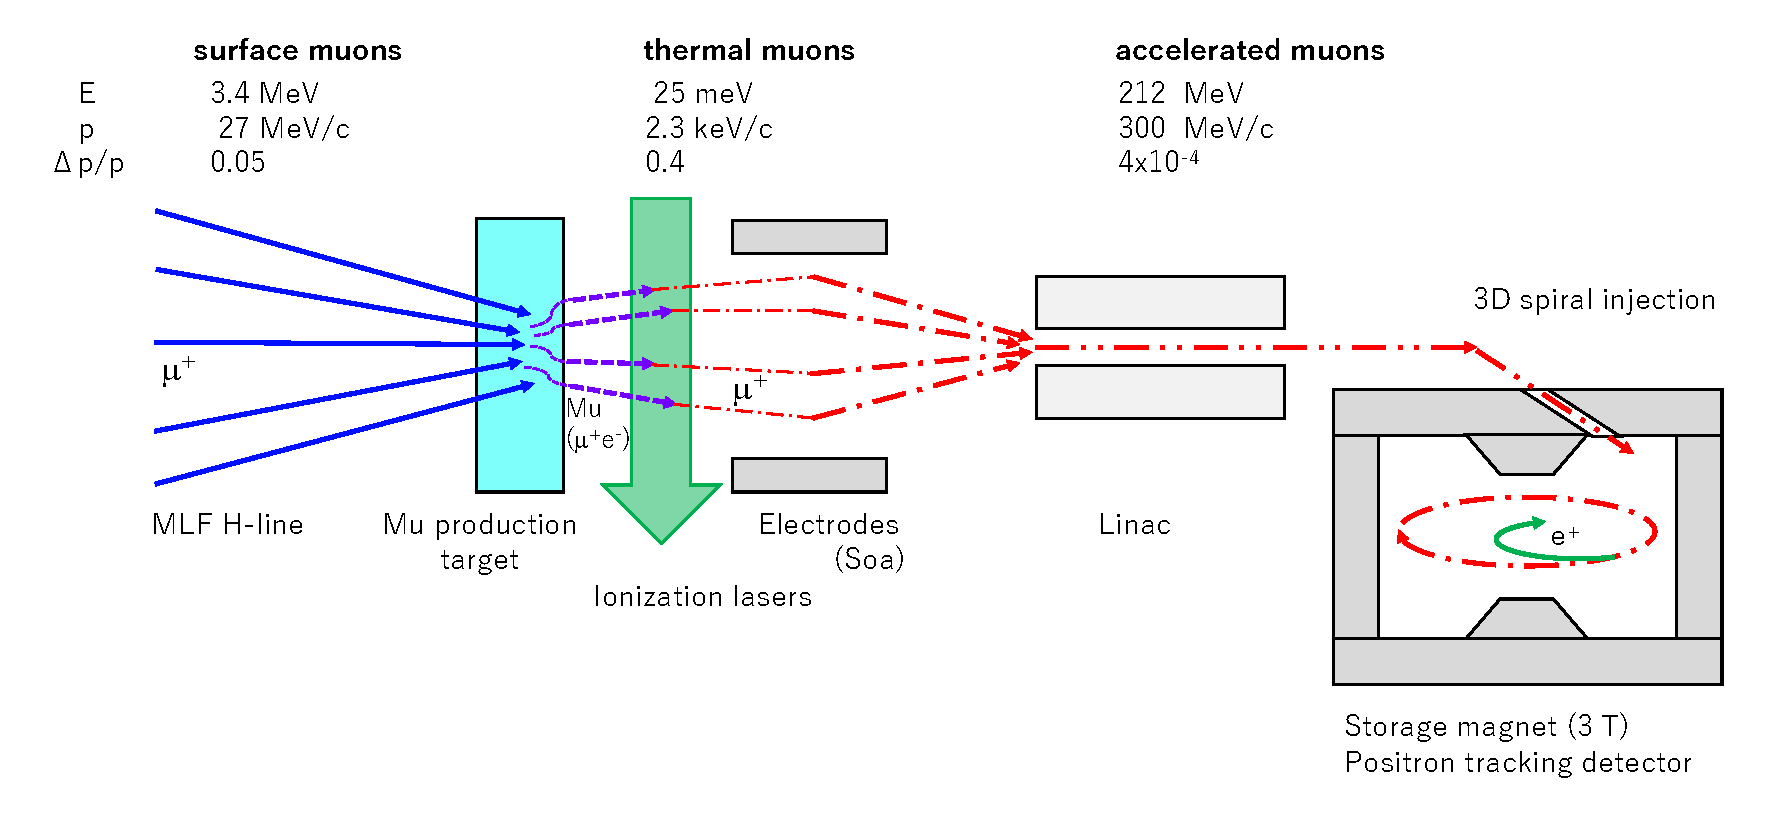
\includegraphics[width=18cm,bb=0 0 850 397]{Fig/muonbeam.pdf}
  \end{center}
  \caption{Schematic of the muon $g-2$/EDM experiment at J-PARC MLF. }
  \label{fig:setup}
\end{figure}

The experiment will be installed at the muon facility~\cite{Higemoto:2017} in
the Materials and Life science Facility (MLF) of J-PARC.
A schematic of the experimental setup is shown in Fig.~\ref{fig:setup}. 
A 3~GeV primary proton beam with 1~MW beam power from the Rapid Cycle Synchrotron hits 
a 2~cm thick graphite target to provide pulsed muon beams.
The proton beam has a double-pulse structure, and each pulse is 100~ns in FWHM 
with a 600~ns separation and 25~Hz repetition rate.
The experiment uses a surface muon beam.
Surface muons are 100\% polarized positive muons from pions 
stopped at and near the target surface with the consequent momentum of 29.8 MeV/$c$ and below.
There are four beamlines extracting muon beams.
The experiment will use one of those, the H-line~\cite{Kawamura:2018apy}.
The intensity of the surface muon beam at H-line is estimated 
to $10^8$ per second at the designed proton beam power of 1 MW.
The surface muon at the end of the beamline has a momentum centered at 28.2 MeV/c with 
10\% momentum bite.

The surface muon beam is converted at its final focus into a
source of room-temperature muons. The first step is to
slow and thermalize the $\mu^{+}$ in a carefully selected
material, silica aerogel \cite{Tabata:2011aa}.  In this
material, most of the muons form muonium atoms ($\mu^{+}e^{-}$, or Mu)
that diffuses as a neutral atom into a vacuum region where Mu is
ionized by laser excitation.
The emission of Mu from aerogel has been discovered and verified by experiments
on a surface muon beam line at TRIUMF~\cite{Bakule:2013poa,Beer:2014ooa} and J-PARC.
The emission probability was enhanced by an order of magnitude if the
downstream aerogel surface was covered with a close-packed array of holes
produced by laser ablation to a depth of order a few mm. 
The 50\% polarization is the maximum after statistical spin
distribution among hyperfine states in the Mu atom.

The region of laser ionization is defined as a volume of $40\times 40\times 5$~mm$^3$ in the transverse directions,
and the longidudinal direction, respectively.
A high-power ionizing laser beam system is synchronized to the
periodic 25~Hz thermal Mu production at its maximum density in vacuum.
One laser at 122~nm (Ly-$\alpha$) with 80~GHz linewidth and 100~$\mu$J per pulse excites the Mu from the $1s$ atomic state
to $2p$, then a second at 355~nm with 300~mJ strips the electron. 
The generation of coherent Ly-$\alpha$ light is realized by using a nonlinear conversion process 
of the two-photon resonance four-wave difference frequency mixing in Kr gas~\cite{laser:2016}.
The feed lights are generated by a solid state laser system consisting of 
a fiber coupled distributed feedback laser diode followed by
three stages of amplification and nonlinear conversions.

%=========================================================
%\subsection{Acceleration}

%%%%%%%%%%
%Overview
%%%%%%%%%%

The thermal muons created in the laser ionization of thermal muonium is
accelerated to a momentum of 300~MeV/$c$ (212~MeV in kinetic energy).
The muons must be accelerated in a sufficiently short time
compared with the muon life time of 2.2~$\mu$s
to suppress muon decay loss during the acceleration.
Another essential requirement for the acceleration is
the suppression of transverse emittance growth.
To satisfy these, a linac dedicated to this purpose will be used in the experiment.
Figure~\ref{fig:mulinac_config} shows the schematic configuration
of the muon linac.
In accelerating the muons, the $\beta$ increases rapidly with the kinetic energy.
It is important to adopt adequate accelerating structures to obtain high acceleration efficiency,
similar to proton linacs. 
There are five acceleration steps by using electrostatic acceleration with a Soa lens,
radio frequency quadrupole (RFQ),
inter-digital H-type drift tube linac (IH-DTL)~\cite{Otani:2016swo},
disk-and-washer structure (DAW),
and disk-loaded traveling wave structure (DLS).
Accelerating negative muonium ion to 90~keV by using a RFQ
was successfully demonstrated~\cite{Bae:2018atj}.
A several types of beam monitors for low-energy and low-intensity muon beam have been
developed with a MCP~\cite{Kim:2018aah} and a thin CsI foil.

\begin{figure}[t]
\centering
\includegraphics*[width=1.0\textwidth,bb=0 0 680 170]{Fig/muonlinac.pdf}
\caption{Schematic configuration of the muon linac. Figure from~\cite{TDRsummarypaper}.}
\label{fig:mulinac_config}
\end{figure}

%===============================================================
%\subsection{Beam injection and muon storage magnet}

The muon beam is injected into the muon storage magnet. 
Due to the limited space of the storage magnet, 
the muon beam is not injected by the previous method used for CERN, BNL and Fermilab $g-2$ experiments 
of horizontal injection using an inflector magnet with poor ($2\sim5\%$) efficiency. 
Instead, a new $3$-D spiral injection scheme~\cite{Iinuma:2016zfu} is developed.
The muon beam follows a beam transport line to inject the muon 
beam at an incident vertical angle of 25~degrees. The beam transport line consists of 
two dipole magnets for bending the beam vertically, three normal quadrupole magnets
to match the vertical momentum dispersion and eight rotated quadrupole magnets
to control the phasespace to match the acceptance of injection into the magnet.

\begin{figure}[t]
%\vspace*{-0.3cm}
%\vspace*{7.0cm}
 \centerline{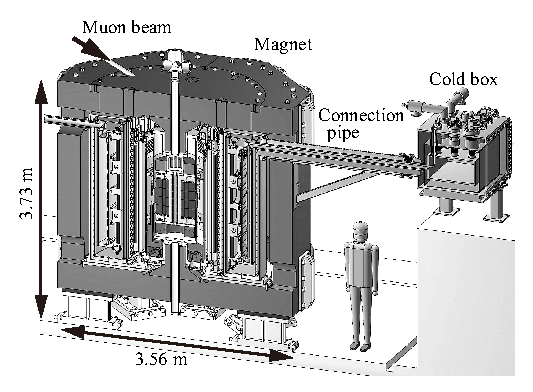
\includegraphics[width=12cm]{Fig/MagnetMechOverviewBW.eps}}
 \caption{Overview of the muon storage magnet. Figure from Ref.~\cite{TDRsummarypaper}.}
\label{fig:magdesign}
%\vspace*{-0.3cm}
\end{figure}

A $3$~T MRI-type superconducting solenoid magnet will be used to complete the injection and store the muon beam.
Figure~\ref{fig:magdesign} shows an overview of the muon storage magnet~\cite{Sasaki-etal-IEEE}.
The muons are stored in a 3~T magnetic field with a cyclotron radius of $333$~mm.
The magnet system provides four types of magnetic field; a high uniform storage,
the injection field, the pulsed kicker field to store the muons, weak focusing for storage~\cite{Abe:2018tmp}.

A highly homogeneous magnetic field of $3$~T is produced
in the central region of the magnet, the storage region, where the muon beam is stored until its decay. 
The homogeneity of magnetic field in the storage region is directly related to the sensitivity of the $g-2$ measurement.
The integrated magnetic main field uniformity along the beam orbit in the storage region has to
be carefully controlled with a precision of $100$~ppb peak-to-peak.
The relative field distribution in the r-z plane around the storage region, averaged over the muon orbit has a variation less than $\pm 50$~ppb. 
This field uniformity is a feature of this experiment; the field variation along the muon orbit for the BNL~(E$821$) magnet was as large as $\pm$~100 ppm.

In the injection region, the radial component, $B_{r}$, of the magnetic field has to be carefully controlled from the top end of the magnet to the storage region for smooth injection. 
A three-dimensional view of beam trajectories from the injection region to the storage region is also shown in the right side. 
The muon beam enters from a downward with injection angle (pitch angle) of $440$~mrad. 

The pulsed kicker field makes a vertical kick to the muon beam, guiding the beam towards the storage region.
Two pairs of one-turn coils, the kicker coils at $\pm0.4$~m in height, 
generate a pulsed radial field $B_{kick}$ to apply a vertical kick to the muon beam motion. 
The vertical beam motion from the start of the kick to the end, as well as the beam motion in the storage region.

The weak focusing magnetic field~\cite{Iinuma:2016zfu} keeps the beam in a stable orbit,
The equations of the weak focusing magnetic field are 
\begin{eqnarray}
 B_r &=& -n\frac{B_{0z}}{R}z, \\
 B_z &=& B_{0z}-n\frac{B_{0z}}{R}(r-R)+ n\frac{B_{0z}}{2R^2}z^2,  
\label{eq:weak}
\end{eqnarray}
where, $B_{0z}$ (3~T) is the field strength in the $z$ direction at the center of the storage region,
$R$ (333~mm) is the average radius of the stored beam, $n$ is the field index.
The field index is set to $n=1.5\times 10^{-4}$.

The magnetic field is measured by a system with the NMR (nuclear magnetic resonance) method.
To obtain the average magnetic field $\omega_{p}$ experienced by the muon beam,
the magnetic field is measured along the muon storage orbit (integrated) with a precision below 100 ppb level
in the main field of 3~T where local field homogeneity is 1,000 ppb level.
A continuous wave type (CW) NMR will be used in this experiment. 
The resonant absorption signals of protons in water samples is observed
by using a fixed frequency source and a small sweeping magnetic field.
The magnetic field in the storage region will be mapped by scanning the probe with moving stages.
The stages are driven by ultrasonic motors, which can work in the strong magnetic field.
The ultrasonic motors have encoders so that the position of NMR probe is controlled
with a precision of below 0.1~mm.

%===============================================================
%\subsection{Positron Detector}\label{sec:detector}

The positron detector is installed inside of the storage magnet
and measures positron tracks from decay of stored muon beam.
A muon with the momentum of 300~MeV/$c$ circulates with a radius
of 333~mm and decays to a positron, a neutrino and an anti-neutrino
with the life time of 6.6~$\mu$s. The cyclotron period is 7.4~ns.
Since the anomalous precession period is 2.2~$\mu$s, muons circulate
the ring about 300 times on average during one revolution of muon spin.
The goals of the detector are to measure $\omega_{a}$
and the up-down asymmetry of positron direction due to EDM.

Since the muon decay breaks parity, high-energy decay positrons tend to be emitted
in the direction of muon spin~\cite{Michel:1949qe}. By measuring high energy positrons
selectively, positrons emitted forward can be selected and
the time variation of muon spin with respect to the muon momentum direction
can be measured. The sensitivity becomes maximum when positrons
with momentum above 200~MeV/$c$ are counted.

Positrons emitted within the 3~T magnetic field move in a spiral orbit.
This trajectory is detected by radially arranged silicon strip sensors.
Layout of the detector is shown in Fig.~\ref{fig:Detector_overview}. 

\begin{figure}[t]
  \begin{center}
    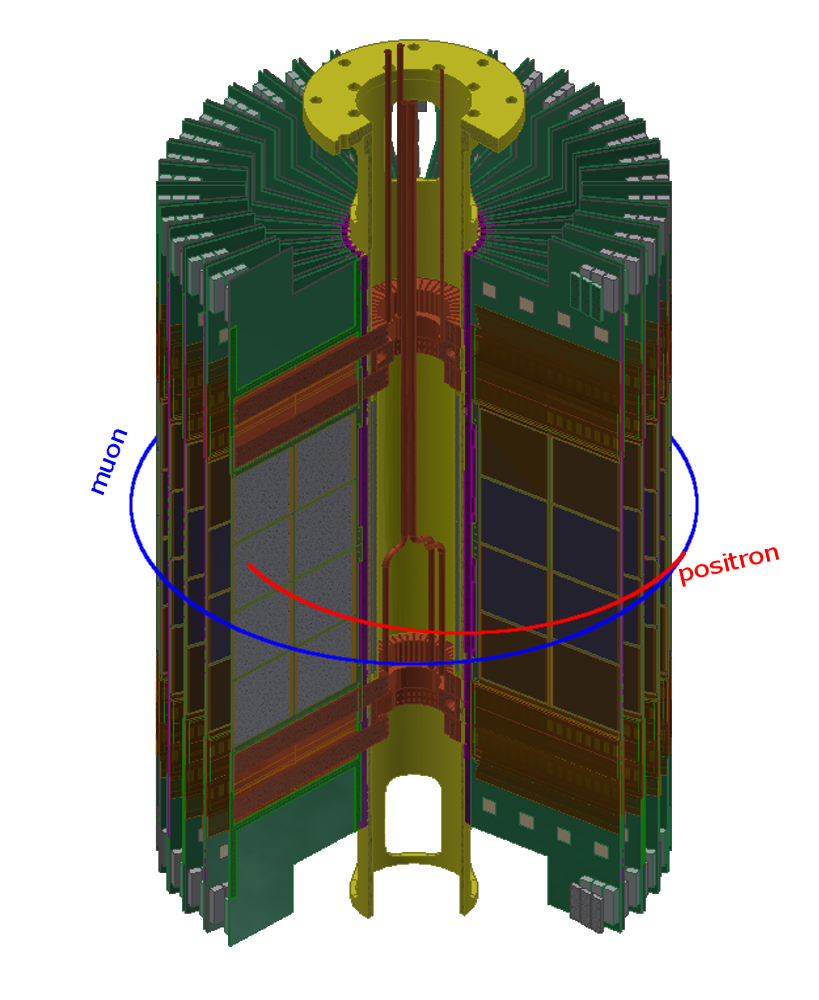
\includegraphics[width=0.4\textwidth, bb=0 0 393 511]{Fig/Detector_cutview.png}
    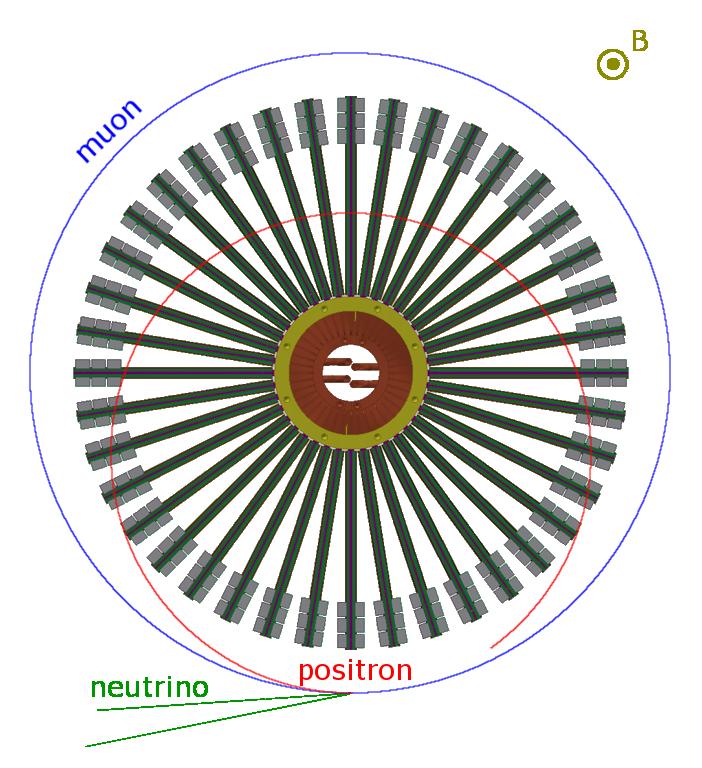
\includegraphics[width=0.4\textwidth, bb=0 0 337 369]{Fig/Detector_topview.png}
    \caption{Perspective view (left) and top view (right) of the positron detector. Figure from Ref.~\cite{TDRsummarypaper}.}
    \label{fig:Detector_overview}
  \end{center}
\end{figure}

Muon beam spill rate is 25~Hz and the number of muons per spill is about $10^4$.
The measurement will be performed in the period of 33~$\mu$s, which is
five times larger than the muon life time. The rate of positrons
changes by a factor of 160 from the beginning to the end of the measurement.
Thus, the detector is required to be stable against the change of positron rate;
otherwise, the measured $\omega_a$ would be biased.

The detector consists of 40 radial modules called vanes.
Each vane consists of 16 sensors.
Sensors are made by single-sided p-on-n technology.
The active area of a sensor is 97.28 mm $\times$ 97.28 mm with
a thickness of 0.32~mm.
A sensor has two blocks of 512 strips and the number of strips
with 190~$\mu$m pitch.
The data acquisition system based on DAQ-Middleware~\cite{daqmiddleware} is used.

A dedicated frontend ASIC is developed~\cite{Tsutsumi:2019ffq}.
Dynamic range of input charge is required to be greater than
4 minimum ionizing particle (MIP) equivalent with linearity.
Equivalent noise charge is required to be less than 
1600~e$^{-}$ with the input capacitance of 30~pF, which
corresponds to the signal-to-noise ratio greater than 15
for a 1~MIP signal. Pulse width at 1~MIP charge is required to
be less than 50~ns and the time-walk between 0.5~MIP and 3~MIP
is required to be less than 5~ns to constrain a timing shift effect
due to pileup hits.

The system clock is provided by the GPS-synchronized Rb frequency
standard, and it is distributed with real time control signals
to the readout boards and the front-end board through the timing
control/monitor board. Long term stability of the system clock
frequency is confirmed better than $10^{-11}$.

The stringent requirement on the detector alignment comes
from the EDM measurement~\cite{EDM_requirement}. Alignment accuracies of vanes
with respect to the magnetic field direction
are required to be better than 10~$\mu$rad for skew, that is an
angle around an axis normal to the vane. 
In order to ensure the required accuracies, alignment changes for the
vanes are detected and monitored during operation using an absolute
distance interferometer system.

At the beginning of spill, about 30 positrons are produced from muon decay in 5~ns which is one time window of the data taking.
The maximum hit rate per silicon sensor strip is $7 \times 10^{-3}$ per time stamp.
Positron tracks are reconstructed from hits by using algorithm based on
the Hough transformation and a Kalman filter.
With this algorithm, track reconstruction efficiency
greater than 90\% is achieved in the positron energy range of
200~MeV$<E<$275~MeV even at the highest positron rate.

%===============================================================
%\subsection{Estimation of number of reconstructed positron}\label{sec:Intensity} 
%Efficiencies of steps from the surface muon production to the detection of positrons are studied 
%by a chain of simulations.
%The simulations include the surface muon production,
%thermal muon production, reacceleration, injection to the muon storage
%magnet, muon beam dynamics in storage, and ended by the detection of the positron.
%The simulation of surface muon production~\cite{otani:simulation_usm_production:ipac2018}
%and thermal muon production are optimized by the experimental data
%on surface muon yield at the existing beamline and measurements of muonium space-time distribution~\cite{Beer:2014ooa},
%respectively.
%Total efficiency is $1.4 \times 10^{-5}$ per initial muon at production.
%At the proton beam power of 1~MW, the expected number of positrons is $5.7 \times 10^{11}$ for $2 \times 10^7$ seconds data taking.

%\subsection{Extraction of $a_{\mu}$ and EDM}\label{sec:Sensitivities} 

The $\omega_a$ and $\eta$ are obtained from the muon decay time distribution.
The muon decay time is reconstructed from the positron track.
A simulated time spectrum for detected positrons in the energy range 
between 200~MeV and 275~MeV is shown in Fig.~\ref{fig:Wiggle}~(left).
The anomalous precession frequency $\omega_a$ is extracted by fitting to the data. 
Alternatively, one can make a ratio of 
data taken with different initial spin orientations.
This will be useful to study early-to-late changes in the detector performance.

\begin{figure}[t]
  \centering
    \begin{tabular}{c}

      \begin{minipage}{0.5\hsize}
        \centering
        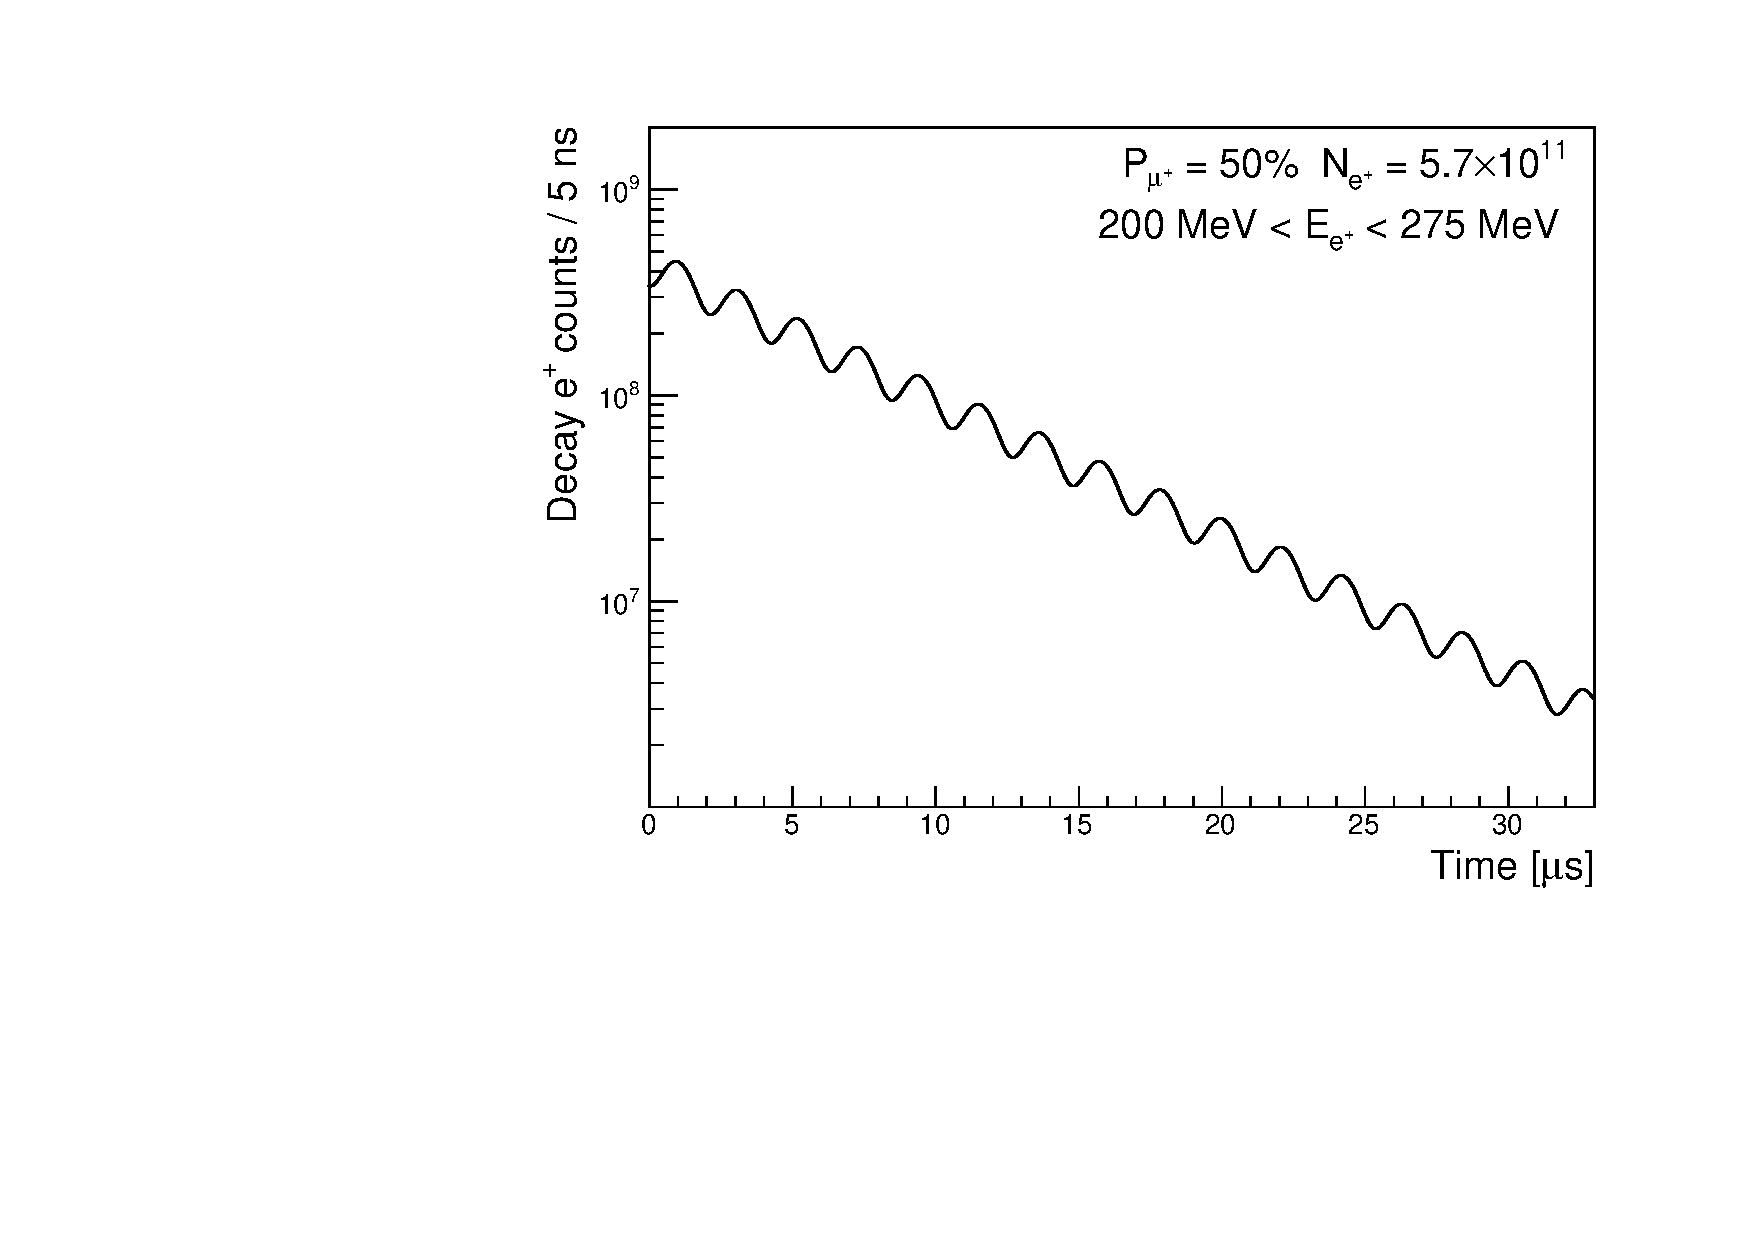
\includegraphics[width=0.7\linewidth, angle=270, bb=20 255 428 822]{Fig/WigglePlot.pdf}
      \end{minipage}

      \begin{minipage}{0.5\hsize}
        \centering
        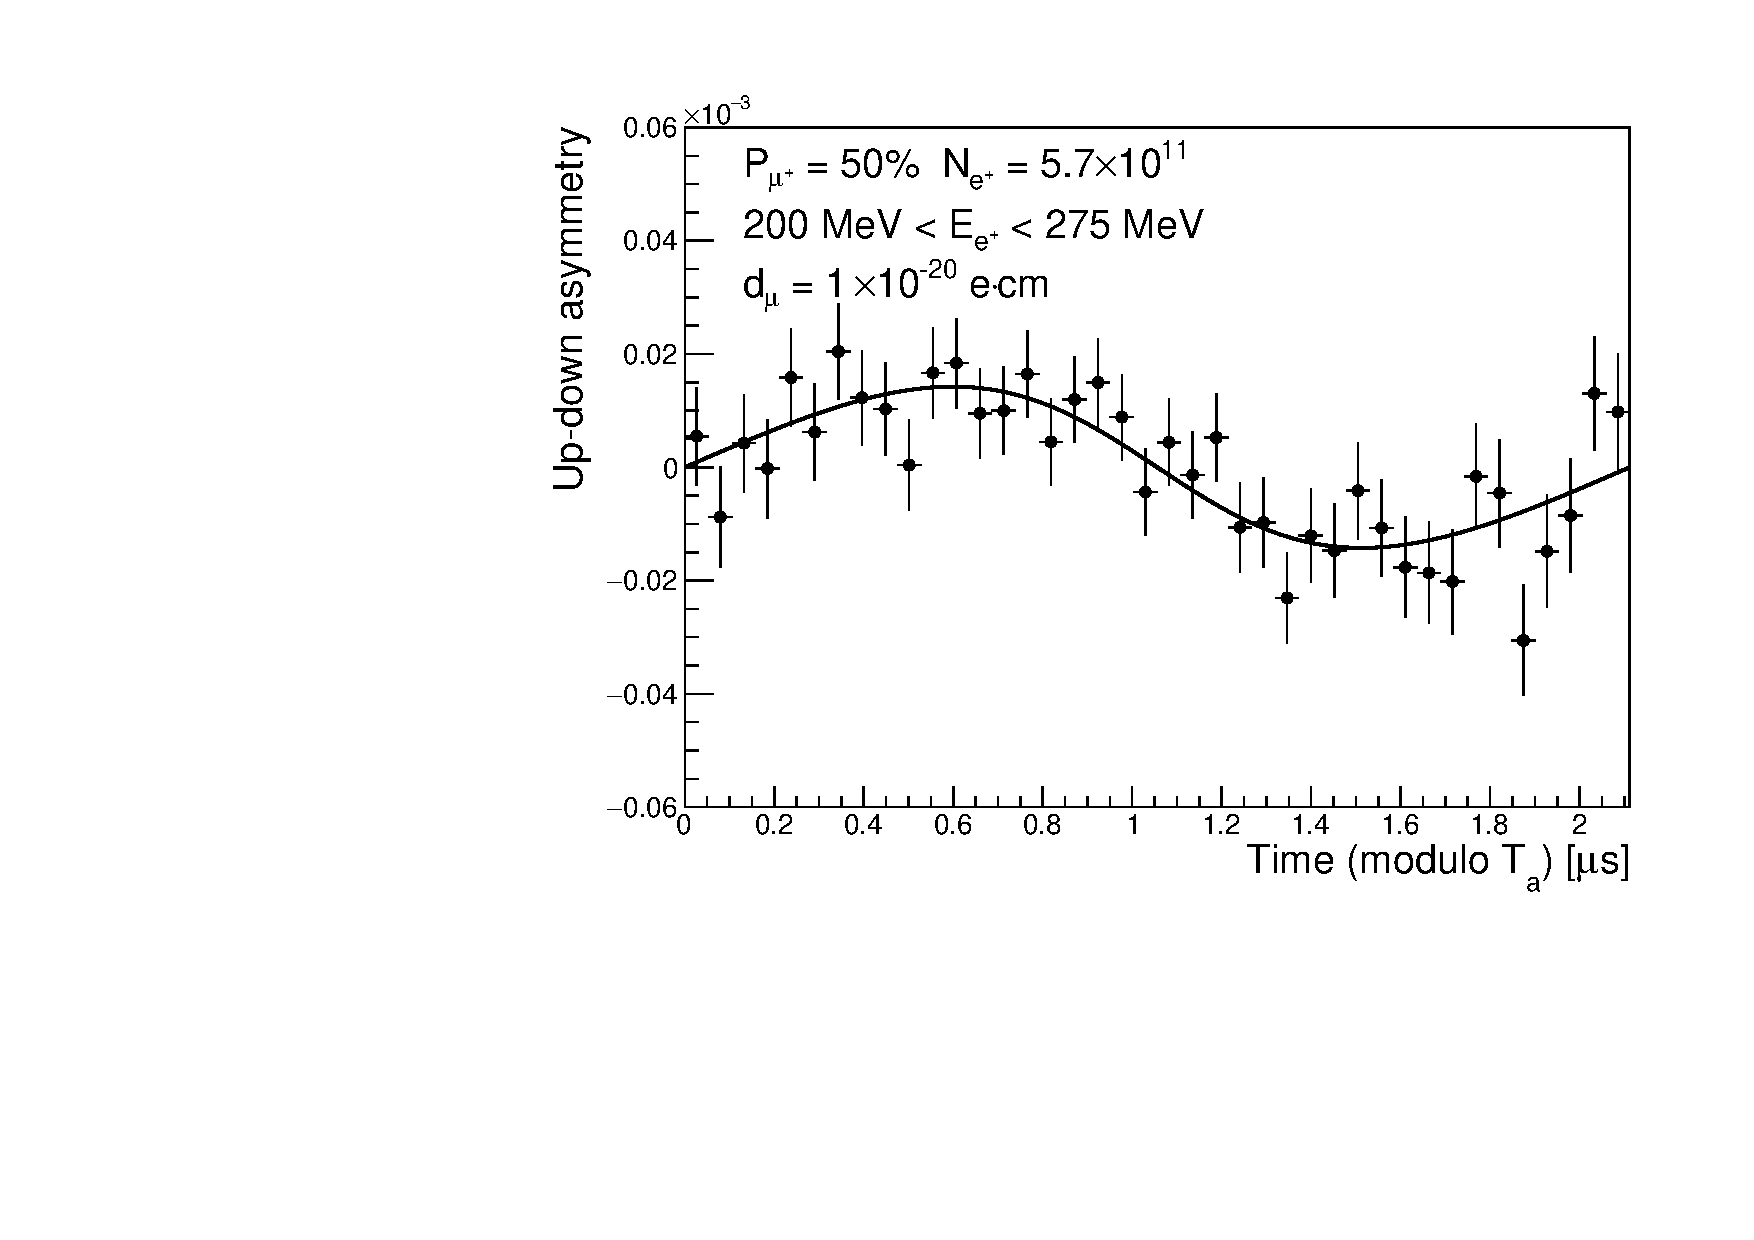
\includegraphics[width=0.7\linewidth, angle=270, bb=20 255 428 822]{Fig/EDMModuloPlot_20_40.pdf}
      \end{minipage}
    \end{tabular}

    \caption{Simulated time distribution of reconstructed positron (left) 
      and the up-down asymmery as a function of time modulo of the $g-2$ period (right).
      Solid curve is the fit to data. Figure from Ref.~\cite{TDRsummarypaper}.}
    \label{fig:Wiggle}
\end{figure}

The $\omega_p$, average magnetic field seen by the muons in the storage ring, is 
measured by independent measurements of the magnetic field map in the storage ring provided from the proton
NMR data and the muon beam distribution deduced from tracing back the positron track to the muon beam.
A blind analysis will be done as was done by the previous BNL expriment, separating the results for 
magnetic field and sipin precession until all systematic uncertainties are finalized.

Once the $\omega_a$ and $\omega_p$ are extracted from the experimental
data, $a_\mu$ is obtained from Eq.~\ref{eq:amu}.
Table~\ref{tab:sensitivity} summarizes statistics and uncertainties for $2 \times 10^7$ seconds of data taking.
The estimated statistical uncertainties on $\omega_a$ and $\omega_p$ are 450~ppb and 100~ppb,
respectively. Thus, the statistical uncertainty of $a_{\mu}$ would be 460~ppb.

Systematic uncertainties on $\omega_a$ are estimated as follows.
A timing shift due to pile up of hits in the tracking detector is estimated as less than 36~ppb
in the detector simulation by taking into account time responses of readout electronics.
A correction for pitch angle is not necessary in the case of the muon storage 
in the perfect weak magnetic focusing field~\cite{Semertzidis:2016kte}. 
A difference in the actual field distribution 
from the perfect case leads to a systematic uncertainty of 13~ppb which is estimated from a precision spin-tracking simulation
of the muon beam storage.
Residual electric field modifies $\omega_a$ through the $\beta \times E$ term. 
With 1~mV/cm monitoring resolution for an E-field, the error on $\omega_a$ is 10~ppb. 
Other effects, such as delayed high-energy positrons and differential decay, are 
of the order 1~ppb.
 In the $\omega_p$ measurement, absolute calibration of the standard probe has an uncertainty of 25 ppb.
Positioning resolution of the field mapping probe at the calibration point and the muon storage
region leads to 20~ppb and 45~ppb uncertainties, respectively.
Other effects, such as field decay and eddy current from kicker are less than 10~ppb.
In summary, we estimate that the combined systematic uncertainties on $a_{\mu}$ is less than 70~ppb.

\begin{table}[t]
  \caption{Summary of statistics and uncertainties}
  \label{tab:sensitivity}
  \begin{center}
%  \begin{small}
  \begin{tabular}{|p{0.5\textwidth}|c|c}
  \hline
          & Estimation \\
    \hline
    \hline
%    Running time [s] & $2\times 10^{7}$ \\
%    Muon beam polarization & 0.5 \\ 
%    Average muon rate in the storage magnet [s$^{-1}$] & $2.6\times 10^{5}$ \\
    Total number of muons in the storage magnet & $5.2 \times 10^{12}$ \\
%    Energy range of $e^{+}$ [MeV] & [200,275] \\
%    Acceptance of the $e^{+}$ & 0.121 \\
%    Track reconstruction efficiency & 0.9 \\
    Total number of positrons &  $5.7\times 10^{11}$ \\
    Effective analyzing power &  0.42 \\
    \hline
    Statistical uncertainty on $\omega_{a}$ [ppb]  &  450 \\
    Statistical uncertainty on $\omega_{p}$ [ppb]  &  100 \\
    \hline
    Uuncertainties on $a_{\mu}$ [ppb]  & 460 (stat.) \\ 
                                                            & $<70$ (syst.) \\
    \hline
    Uncertainties on EDM [$10^{-21}~e\cdot$cm]  & 1.4 (stat.) \\
                                                                              & 0.36 (syst.) \\
    \hline
  \end{tabular}
%  \end{small}
  \end{center}
\end{table}

 A muon EDM will produce muon spin precession out of
the horizontal plane that is defined by the ideal muon orbit.
This can be seen from Eq.~\ref{eq:omega_tot}
where the second term is the EDM term that is perpendicular
to the $a_\mu$ term. Due to the fact that the EDM term generates
vertical motion of the spin, one can extract the EDM term
from the oscillation of the up and down asymmetry $\mathcal{A}_{UD}(t)$ in
number of positrons detected,
\begin{eqnarray}
\mathcal{A}_{UD}(t) = 
\frac{N^{up}(t) - N^{down}(t)}{N^{up}(t) + N^{down}(t)} =
\frac{PA_{EDM} \sin{(\omega_{tot}t+\phi)}}{1+ P A \cos{(\omega_{tot}t+\phi)}},
\end{eqnarray}
where $P$ and $A$ are the polarization of the muon and an effective analyzing power of muon decay, respectively. $A_{EDM}$ is an effective analyzing power associated with the EDM.
A simulated up-down asymmetry in the case of $d_{\mu}=1\times 10^{-20}~e\cdot\mbox{cm}$ 
is shown in Fig.~\ref{fig:Wiggle}~(right).
The estimated statistical sensitivity for EDM is $1.5\times 10^{-21}~e\cdot\mbox{cm}$ (See Table~\ref{tab:sensitivity}).

A major source of systematic uncertainties on EDM is detector misalignment with respect to
the plane of the muon storage. The alignment resolution is estimated as 
$0.36\times 10^{-21}~e\cdot\mbox{cm}$ from the resolution 
of the alignment monitor system made with an optical frequency comb technology.
Effects of axial electric field and radial magnetic field~\cite{Silenko:2017vvd}
are both less than $10^{-24}~e\cdot\mbox{cm}$, thus negligibly small.

%===============================================================
%\subsection{Summary and prospects}\label{sec:Summary} 

In summary, a new method of measuring $a_{\mu}$ and EDM of the muon is described.
This experiment intends to reach statistical uncertainties for $a_{\mu}$ of 460~ppb and for muon EDM of
$1.5\times 10^{-21}~e\cdot\mbox{cm}$, for an acquisition time
of $2 \times 10^7$ seconds. The statistical precision is comparable to
that of the BNL experiment. The EDM sensitivity is about two orders of magnitude
smaller than the BNL limits.
Estimated systematic uncertainties on $a_{\mu}$ and EDM are
factor of seven and four smaller than the statistical uncertainties, respectively.
At present, experiment is statistically limited, but 
will test the 3~$\sigma$ deviation on $g-2$ reported by
the BNL E821 experiment with significantly different and improved systematic uncertainties 
and search for new sources of T-violation in the muon with unprecedented sensitivity.

The experiment was officially approved for the stage 2 status 
by the institute of particle and nuclear studies and 
the institute of materials and structure science of KEK
as of November 2018 and Ferbruary 2019, resepectively.
